%=======================02-713 LaTeX template, following the 15-210 template==================
%
% You don't need to use LaTeX or this template, but you must turn your homework in as
% a typeset PDF somehow.
%
% How to use:
%    1. Update your information in section "A" below
%    2. Write your answers in section "B" below. Precede answers for all 
%       parts of a question with the command "\question{n}{desc}" where n is
%       the question number and "desc" is a short, one-line description of 
%       the problem. There is no need to restate the problem.
%    3. If a question has multiple parts, precede the answer to part x with the
%       command "\part{x}".
%    4. If a problem asks you to design an algorithm, use the commands
%       \algorithm, \correctness, \runtime to precede your discussion of the 
%       description of the algorithm, its correctness, and its running time, respectively.
%    5. You can include graphics by using the command \includegraphics{FILENAME}
%
\documentclass[11pt]{article}
\usepackage{amsmath,amssymb,amsthm}
\usepackage{graphicx}
\usepackage[margin=1in]{geometry}
\usepackage{fancyhdr}
\usepackage{listings}
\setlength{\parindent}{0pt}
\setlength{\parskip}{5pt plus 1pt}
\setlength{\headheight}{13.6pt}
\newcommand\question[2]{\vspace{.25in}\hrule\textbf{#1: #2}\vspace{.5em}\hrule\vspace{.10in}}
\renewcommand\part[1]{\vspace{.10in}\textbf{(#1)}}
\newcommand\algorithm{\vspace{.10in}\textbf{Algorithm: }}
\newcommand\correctness{\vspace{.10in}\textbf{Output: }}
\newcommand\runtime{\vspace{.10in}\textbf{Running time: }}
\pagestyle{fancyplain}
\lhead{\textbf{\NAME\ (\ANDREWID)}}
\chead{\textbf{Lab\HWNUM}}
\rhead{\today}
\begin{document}\raggedright
%Section A==============Change the values below to match your information==================
\newcommand\NAME{Yao Xiao}  % your name
\newcommand\ANDREWID{2019180015}     % your andrew id
\newcommand\HWNUM{2}              % the homework number
%Section B==============Put your answers to the questions below here=======================

% no need to restate the problem --- the graders know which problem is which,
% but replacing "The First Problem" with a short phrase will help you remember
% which problem this is when you read over your homeworks to study.

\question{1}{The First Problem} 

\part{a} \algorithm\
\begin{lstlisting}
import numpy as np

inputs = np.array([[0,0,1],[0,1,1],[1,0,1],[1,1,1]])
outputs = np.array([0,0,1,1])
w = np.transpose(np.array([0,0,0]))
theta = 0.1
epoch = 2000

for i in range(epoch):
    for j in range(4):
        y_hat=1/(1+np.exp(-np.dot(w,inputs[j])))
        dw=theta*(outputs[j]-y_hat)*y_hat*(1-y_hat)*outputs[j]
        w=w+dw


for j in range(4):
    y_hat=1/(1+np.exp(-np.dot(w,inputs[j])))
    print(y_hat)
\end{lstlisting}

\part{b} \correctness\\
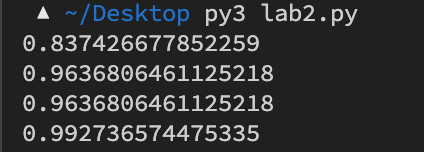
\includegraphics[scale=1]{ot1.png}

\question{2}{The second problem}
\begin{lstlisting}
import numpy as np

inputs = np.array([[0,0,1],[0,1,1],[1,0,1],[1,1,1]])
y = np.array([0,0,1,1])
w = np.transpose(np.array([0,0,0]))
theta = 0.1
epoch = 2000

def sigmoid(x):
    return 1 / (1 + np.exp(-x))

for i in range(epoch):
    for j in range(4):
        y_hat = sigmoid(np.dot(w,inputs[j]))
        dw = theta * (y[j]-y_hat) * y_hat * (1-y_hat) * inputs[j]
        w = w + dw

for j in range(4):
    y_hat = sigmoid(np.dot(w,inputs[j]))
    print(y_hat)


w = np.transpose(np.array([0,0,0]))
y_avg = np.empty([2,3], dtype=float)
for i in range(epoch):
    for j in range(2):
      for k in range(2 * j,2 * j + 1):
          y_hat = sigmoid(np.dot(w,inputs[k]))
          y_avg[j] = (y[k]-y_hat) * y_hat * (1-y_hat) * inputs[k]
    dw = theta * ((y_avg[0] + y_avg[1])/2)
    w = w + dw

for k in range(4):
    y_hat = sigmoid(np.dot(w,inputs[k]))
    print(y_hat)
\end{lstlisting}

\part{b} \correctness\\
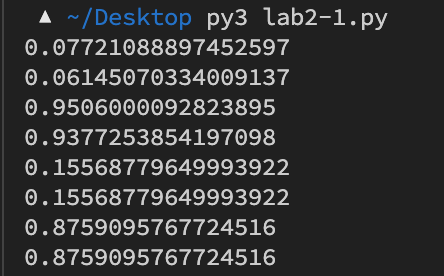
\includegraphics[scale=1]{ot2.png}

\end{document}
